\documentclass[11pt,letterpaper]{article}
\usepackage[margin=0.82in]{geometry}
\usepackage{booktabs,longtable,array}
\usepackage{graphicx}
\usepackage{caption}
\usepackage{hyperref}
\usepackage{xcolor}
\usepackage{float}
\setlength{\parskip}{3pt}
\setlength{\parindent}{2em}
\captionsetup{font=small,labelfont=bf}
\hypersetup{colorlinks=true,linkcolor=black,urlcolor=blue,pdftitle={FewClick Supplementary Material},pdfauthor={Anonymous}}
\graphicspath{{额外可视化/}{额外可视化/TLS30_review_panels/}}
\newcommand{\code}[1]{\texttt{#1}}
\begin{document}

\begin{center}
{\LARGE \textbf{FewClick: Reproducibility Technical Appendix}}\\[5pt]
{\large Anonymous Supplementary Material}
\end{center}

\noindent\textbf{Overview.} This document is a standalone technical appendix for the paper \emph{A Few-Click Interactive Framework for User-Specified Histopathological Tissue Segmentation}. All training, validation, and external evaluations use configurations frozen at the corresponding stage. This file contains no author names, affiliations, absolute data paths, hospital names, or original case identifiers. Executable code, anonymized configurations, and usage instructions are provided separately as the \code{code\_and\_data.zip} code-and-data attachment.

\section{Datasets and Data Splits}
\subsection{Main Development Cohort}
The main experiments use a tissue-segmentation development cohort of 200 H\&E whole-slide images (WSIs). Pixel-level annotations comprise 12 tissue classes: tumor epithelium, tumor stroma, background, necrosis, normal glands, normal stroma, submucosa/serosa, muscle, lymphoid aggregates, mucus, fat, and blood. Background is not treated as a foreground target, and the ignore label is 255.

Splitting is performed at the WSI level, using patient/WSI identifiers as grouping keys: 140 WSIs for training, 30 for validation, and 30 independent WSIs for testing. Regions from the same WSI never cross splits. The test set is not used for model selection or ablation until the architecture, hyperparameters, and thresholds are frozen. All images are indexed at a $10\times$ target magnification. Patches are $512\times512$ pixels with a stride of 512; only candidates with a valid-pixel fraction of at least 0.50 and a tissue fraction of at least 0.30 are used.

Training samples mix within-class interiors, class boundaries, rare classes, and background/hard negatives at ratios of 0.30/0.30/0.30/0.10. The maximum sampling proportion of rare classes is 0.02, and the boundary-patch threshold is 0.02.

\subsection{External TLS Cohort}
The additional generalization experiment uses 30 H\&E WSIs fully isolated from the main development cohort, with tertiary lymphoid structures (TLS) as the target. TLS is absent from the training label set. This cohort is not used for training, validation, checkpoint selection, or hyperparameter tuning; model parameters remain fully frozen during this experiment.

The 30 WSIs contain 578 TLS polygons in total. Of these, 279 polygons provide positive prompts and 299 are fully held out to measure long-range TLS retrieval driven by local prompts. The prompted/held-out partition is fixed before inference for every WSI.

\section{Prompt Sampling and Evaluation Protocol}
\subsection{Episodic Prompts for the Main Experiments}
An episode consists of a WSI crop, a target tissue class, its binary mask, a set of positive prompts, and an optional set of negative prompts. Each training epoch uses 20,000 episodes; the fixed validation manifest contains 4,000 episodes. Except for the module intentionally removed, ablation variants share the data split, random seed, prompt manifest, data augmentation, and optimization schedule.

Prompt sizes are sampled as point/small-region/large-region at 0.40/0.35/0.25. Prompt locations are sampled from class interiors, class boundaries, rare classes, and background/hard negatives at 0.30/0.30/0.30/0.10. Hard negatives are drawn from adjacent tissues, feature-space neighbors, and high-confidence false-positive regions of the model. The main experiments use three interaction budgets, $(1+1)$, $(3+1)$, and $(5+1)$, corresponding to 1, 3, or 5 positive points plus one negative point.

For WSI-level main experiments, each WSI--tissue task uses one positive and one negative point. Five prompt sets are frozen before inference, and results are summarized as outcome-independent mean $\pm$ standard deviation. If positive and negative prompts map to the same hard region, the prompt conflict is scored as an empty prediction; candidates are not re-selected using ground truth.

\subsection{Prompts and Retrieval Evaluation on External TLS}
For each external WSI, approximately half of the TLS polygons each provide one positive prompt; three negative prompts are sampled from tissue regions without annotated TLS. The remaining TLS polygons do not participate in prompting and serve as held-out retrieval targets. Inference uses the $10\times$ coordinate system, a tile size of 512, a stride of 384, and a downsampling factor of 4 from level-0 to evaluation coordinates.

We report two principal measurements: (i)~\textbf{unprompted-polygon recall}, i.e., whether TLS polygons not used as prompts are retrieved; and (ii)~\textbf{prompt-censored-region metrics}, namely Dice, precision, and recall after removing pixels belonging to prompted TLS from the evaluation domain. Precision and Dice for a single polygon are not used as global quality metrics, because correct predictions of other TLS on the same WSI would be incorrectly counted as false positives under that definition.

\section{Training Configuration and Model Selection}
All stochastic procedures use seeds recorded in the configuration files: 20260714 for Phases 1--2, 20260719 for Phase 3, and 20260720 for Phases 5--6 and TLS inference. The binary threshold at inference is fixed to 0.5.

\footnotesize\sloppy
\begin{longtable}{@{}p{0.12\linewidth}p{0.25\linewidth}p{0.27\linewidth}p{0.25\linewidth}@{}}
\caption{Final configuration at each training stage.}\label{tab:hyperparameters}\\
\toprule
Stage & Model and architecture & Training setup & Optimization and losses\\
\midrule
\endfirsthead
\toprule
Stage & Model and architecture & Training setup & Optimization and losses\\
\midrule
\endhead
Phase 1: $10\times$ visual features & DeepLabV3--ResNet50; 12 classes; $512\times512$ input & 30 epochs; batch size 8 per GPU; 20,000 samples per epoch; 4,000 validation samples; 2 workers/GPU; AMP; gradient accumulation 1; 2-epoch warm-up & LR $10^{-4}$; weight decay $10^{-4}$; cross-entropy/Dice weights 0.5/1.0\\
Phase 2: learnable regions & 64 regions; dimension 256; spatial temperature 0.08; initialized from the Phase-1 checkpoint & 30 epochs; batch size 8/GPU; 20,000/4,000 training/validation samples; bf16 AMP; SLIC retained for 5 epochs and decayed for 15 epochs & Backbone and region-head LR $10^{-5}$ and $10^{-3}$; weight decay $10^{-4}$; gradient clipping 5.0; loss weights for SLIC, boundary, balance, compactness, purity, semantic CE, and semantic Dice: 1.0, 1.0, 0.50, 0.10, 0.25, 0.50, 1.0\\
Phase 3: cell-aware regional representation & At most 255 cells per patch; cell-feature dimension 74; 64 regions, dimension 256; Phase 2 frozen & 30 epochs; batch size 4/GPU; 20,000/4,000 samples; bf16 AMP & LR $10^{-3}$; weight decay $10^{-4}$; gradient clipping 5.0\\
Phase 4: cross-scale interaction & Phases 2--3 frozen; 64 tokens of dimension 256 at each of $10\times$/$5\times$/$2.5\times$; one hierarchical graph block; top-4 physically overlapping parent nodes retained for each child & 30 epochs; batch size 16/GPU; 20,000/4,000 samples; bf16 AMP & AdamW; LR $10^{-3}$; weight decay $10^{-4}$; gradient clipping 5.0; 12-class regional cross entropy (ignore label 255)\\
Phase 5: prompt-set encoding & Region dimension 256; 4 heads; 2 set-encoder layers; dropout 0.10 & 30 epochs; batch size 32/GPU; 20,000/4,000 samples; bf16 AMP & LR $10^{-3}$; weight decay $10^{-4}$; gradient clipping 5.0; Dice/ranking weights 1.0/0.2; margin 0.2\\
Phase 6: final joint model (J5) & Region dimension 256; 4 graph heads; 2 graph layers; 6 neighbors per node; dropout 0.10; KNN=4; only backbone layer 4 unfrozen & 5 epochs; batch size 2/GPU; 20,000/4,000 samples; bf16 AMP & Layer-4 LR $10^{-6}$; preset LRs for parent context, decoder, prompt, Phase-2 embedding, and assignment: $10^{-4}$, $10^{-4}$, $10^{-5}$, $5\times10^{-6}$, $2\times10^{-5}$; weight decay $10^{-4}$; gradient clipping 5.0\\
\bottomrule
\end{longtable}
\fussy\normalsize

\section{Hardware and Software Environment}
Experiments use Linux and the conda environment \code{aligner}. Main training and WSI batch processing use multiple GPUs. External TLS batch inference uses six GPUs (logical indices 0--5), with an inference batch size of 2 and four data-loader workers per GPU. Cell-feature extraction uses one GPU, with XCellFormer batch size 8 and Cellpose network batch size 8. Thread settings are \code{OMP\_NUM\_THREADS=8}, \code{MKL\_NUM\_THREADS=8}, \code{OPENBLAS\_NUM\_THREADS=8}, \code{NUMEXPR\_NUM\_THREADS=8}, and \code{VIPS\_CONCURRENCY=4}.

\begin{center}\small
\begin{tabular}{@{}p{0.29\linewidth}p{0.61\linewidth}@{}}
\toprule
Item & Version/configuration\\ \midrule
GPU & 6 $\times$ NVIDIA RTX 5880 Ada Generation, 49,140 MiB (approximately 48 GiB) per GPU\\
NVIDIA driver / system CUDA & 550.67 / 12.4\\
Operating system & Linux\\
Python & 3.10.19\\
PyTorch & 2.9.1+cu128\\
CUDA runtime & 12.8\\
NumPy & 2.2.6\\
pandas & 2.3.3\\
PyYAML & 6.0.3\\
Cellpose & 4.0.7\\
OpenSlide & 4.0.0 (\code{openslide-python} 1.4.2)\\
pyvips / libvips & 2.2.3 / 8.16.0\\
\bottomrule
\end{tabular}
\end{center}

\section{Additional Quantitative Results: 30 External TLS WSIs}
Results are obtained from the completed 30/30 frozen-model batch evaluation. All values are computed on external data not used during development.

\begin{center}\small
\begin{tabular}{lr}
\toprule
WSI macro average (each WSI equally weighted; mean $\pm$ standard deviation) & Value\\ \midrule
All-TLS union Dice & $0.5229\pm0.2270$\\
All-TLS union precision & $0.4484\pm0.2554$\\
All-TLS union recall & $0.7882\pm0.0836$\\
Unprompted TLS, prompt-censored-region Dice & $0.3955\pm0.2319$\\
Unprompted TLS, prompt-censored-region precision & $0.3139\pm0.2385$\\
Unprompted TLS, prompt-censored-region recall & $0.7675\pm0.1373$\\
Prompted TLS polygon macro recall & $0.7274\pm0.1083$\\
\textbf{Unprompted TLS polygon macro recall} & \textbf{$0.6968\pm0.1479$}\\
Proportion of unprompted polygons with recall $\geq0.1$ & $0.9416\pm0.1278$\\
Proportion of unprompted polygons with recall $\geq0.5$ & $0.7731\pm0.2078$\\
\bottomrule
\end{tabular}
\end{center}

\begin{center}\small
\begin{tabular}{@{}p{0.43\linewidth}p{0.30\linewidth}r@{}}
\toprule
Statistical unit & Metric & Value\\ \midrule
299 equally weighted unprompted TLS polygons & Macro recall & 0.6914\\
299 equally weighted unprompted TLS polygons & Proportion with recall $\geq0.1$ / $\geq0.5$ & 0.9398 / 0.7559\\
299 area-weighted unprompted TLS polygons & Recall & 0.7739\\
Pixel pooling across 30 WSIs, all-TLS union & Dice / precision / recall & 0.2785 / 0.1696 / 0.7785\\
Pixel pooling across 30 WSIs, prompt-censored unprompted TLS & Dice / precision / recall & 0.1719 / 0.0967 / 0.7739\\
\bottomrule
\end{tabular}
\end{center}

Precision and Dice for an individual polygon count predictions of other TLS on the same WSI as false positives, and are therefore not used as principal metrics of global segmentation quality. External generalization is assessed primarily by unprompted-polygon macro recall and WSI-macro averages on the prompt-censored region. Pixel pooling reflects the dominance of large slides in global counts and must not be conflated with WSI-macro averaging.

\paragraph{Generalization to unseen data and an unseen tissue concept.}
The TLS cohort is fully separated from the main development cohort, and TLS is not among the 12 tissue labels used for training. No parameter updates, threshold calibration, or external-cohort-specific prompt optimization is performed at inference. This experiment therefore requires the model to infer the current tissue concept from a small number of local spatial prompts and to retrieve TLS with compatible morphology and histological semantics throughout the WSI, including locations spatially disconnected from prompted regions. Although it has not encountered this data source or TLS as a target tissue, the frozen model completed inference and evaluation on all 30/30 WSIs. Under equal WSI weighting, the macro recall of unprompted TLS polygons is $0.6968\pm0.1479$, while recall remains $0.7675\pm0.1373$ after prompted TLS areas are removed. This finding indicates that the response is not limited to connected regions around clicks, but can transform local prompts into WSI-wide tissue-retrieval cues.

At the finer held-out-polygon level, 93.98\% of the 299 unprompted TLS polygons achieve recall of at least 0.1, and 75.59\% achieve recall of at least 0.5; the area-weighted recall is 0.7739. This high recall coverage indicates that the model provides candidate regions suitable for subsequent interactive refinement for most TLS that did not participate in prompting. At the same time, Dice and precision are more sensitive to external staining, tissue-background differences, and broad candidate areas within a slide. Accordingly, this experiment supports \emph{few-shot cross-dataset retrieval of an unseen tissue concept}, rather than a claim of fully open-world TLS segmentation without interaction.

\section{Additional Visualizations}
\begin{figure}[H]
\centering
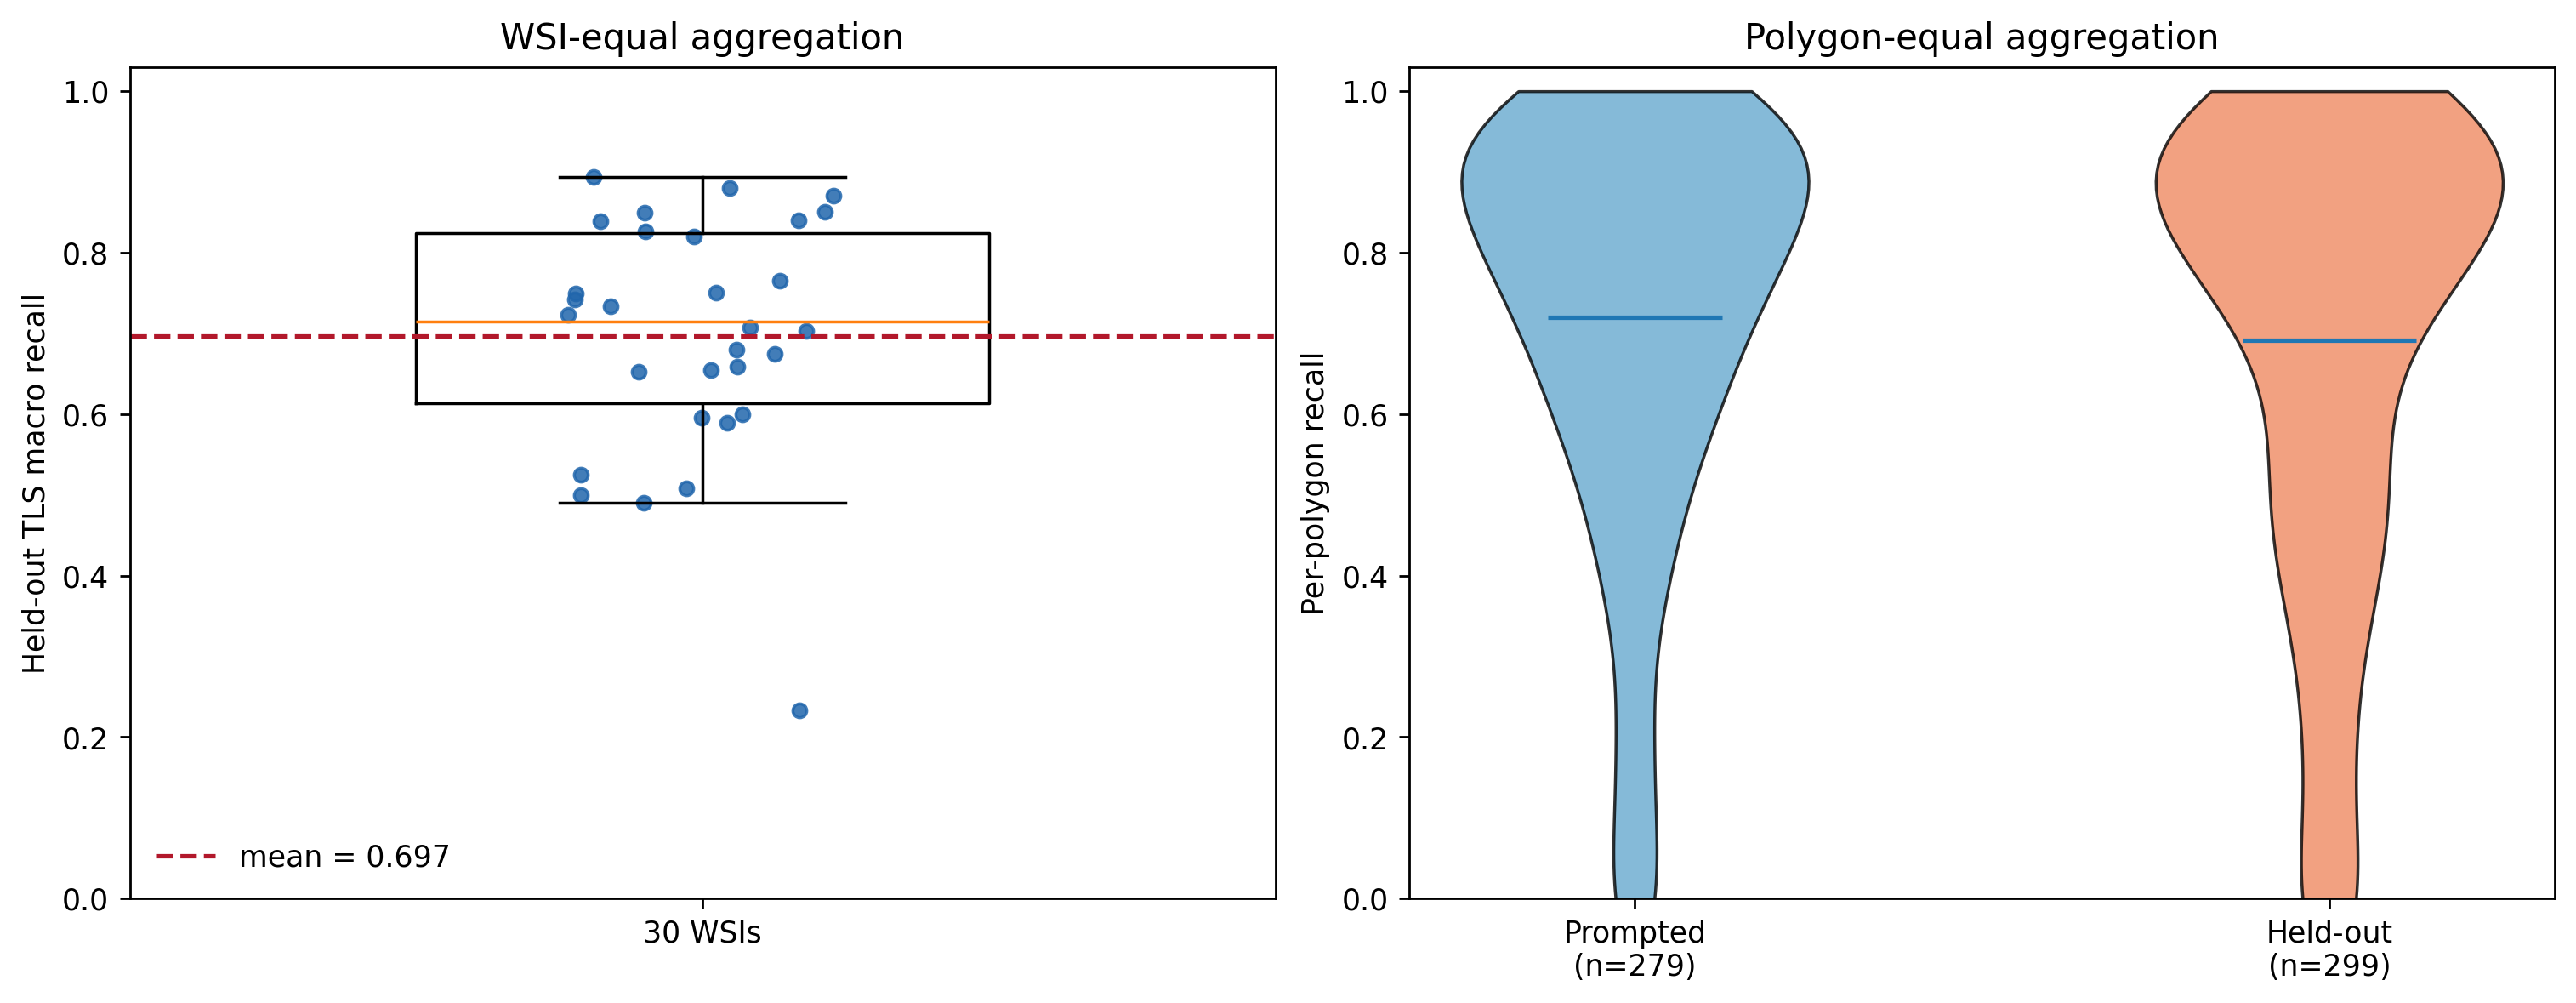
\includegraphics[width=\linewidth]{TLS30_retrieval_recall_distributions.png}
\caption{Recall distributions for external TLS retrieval. Left: unprompted-TLS macro recall with equal weighting of the 30 WSIs. Right: equally weighted recall for prompted ($n=279$) and held-out ($n=299$) TLS polygons. The two panels use different statistical units.}
\label{fig:tls-distribution}
\end{figure}

\begin{figure}[H]
\centering
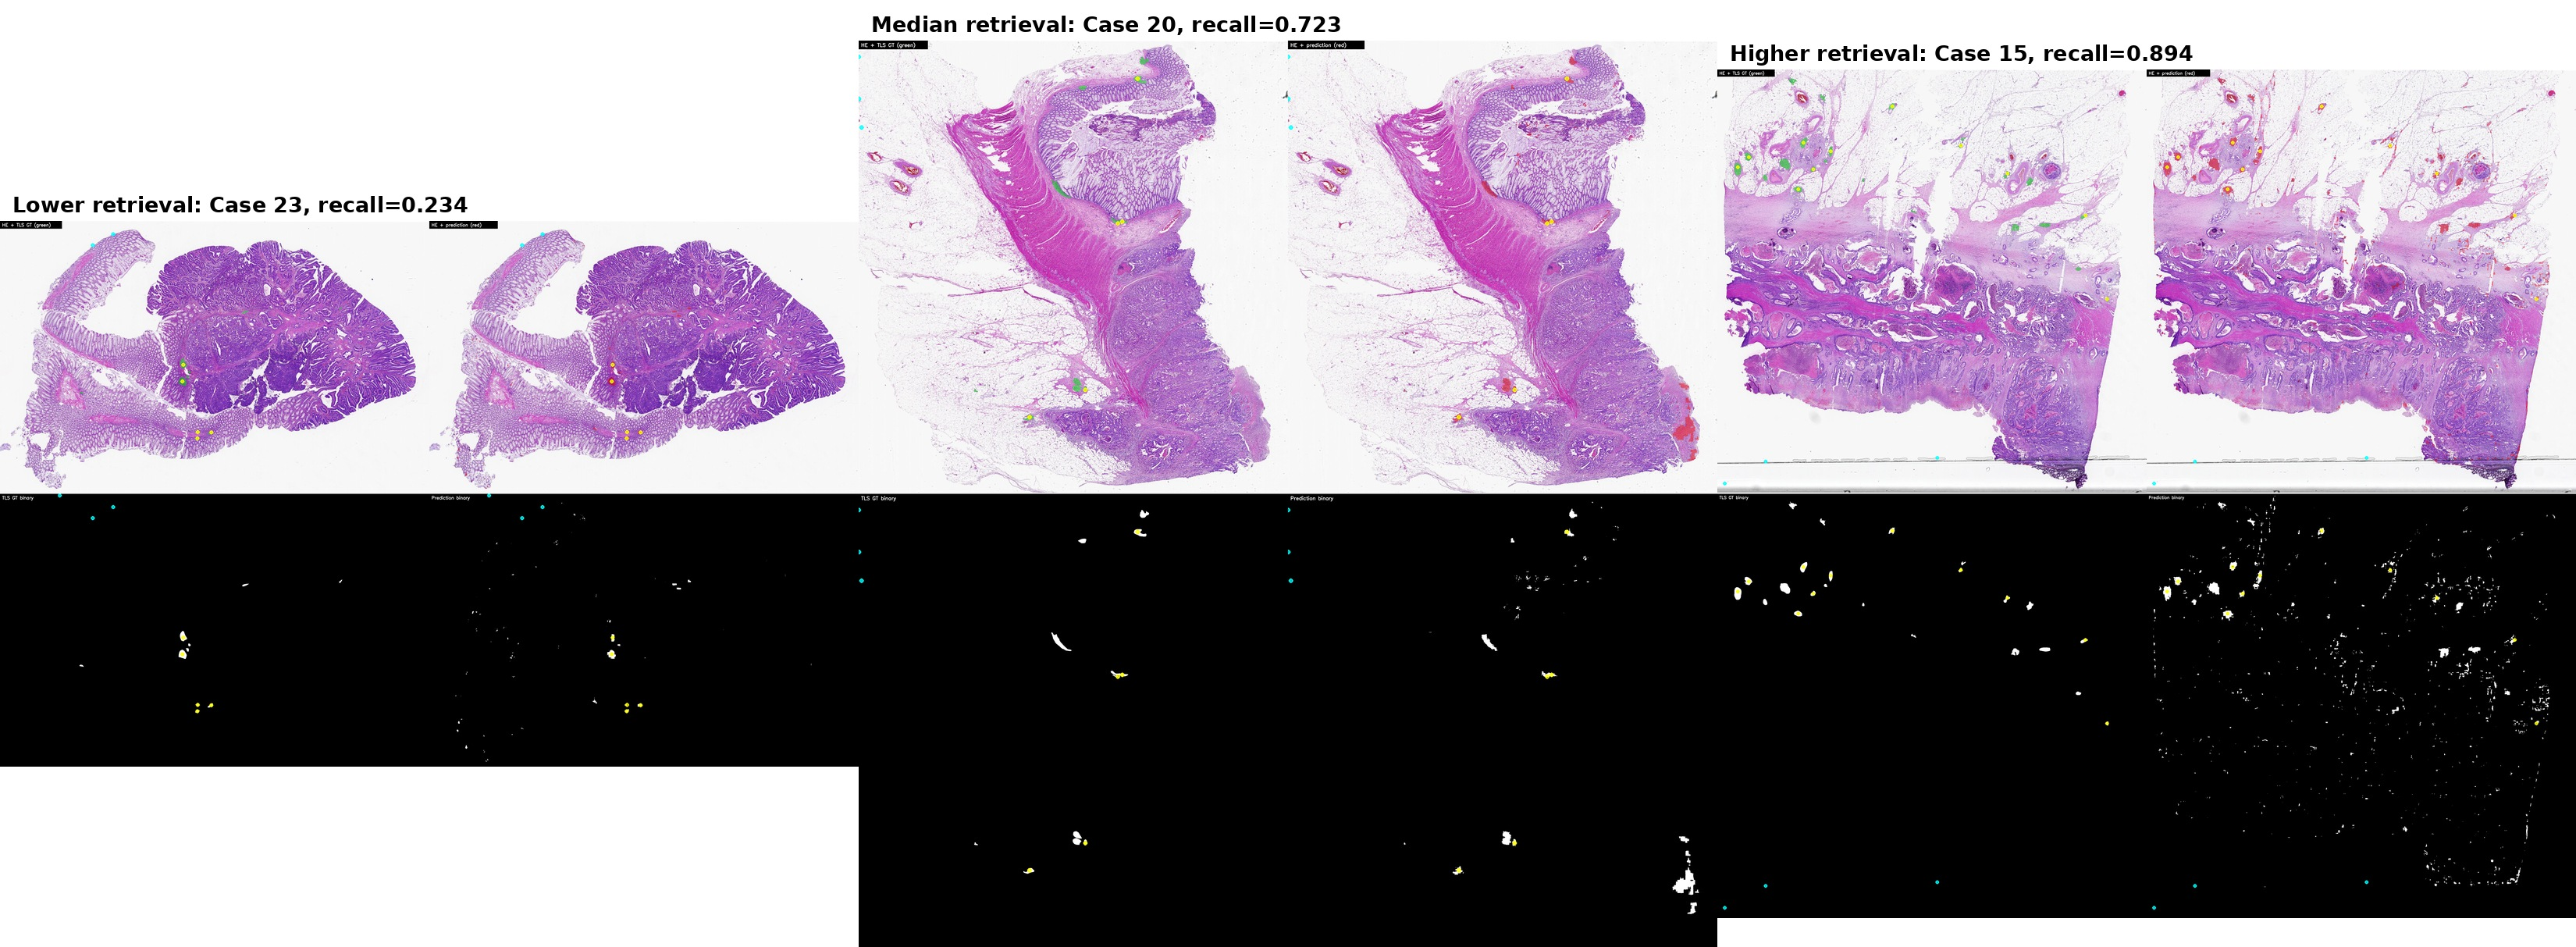
\includegraphics[width=0.97\linewidth]{TLS30_representative_retrieval_cases.jpg}
\caption{Representative low-, middle-, and high-retrieval cases selected automatically by unprompted-TLS macro recall. Each four-panel case shows H\&E with TLS ground truth, H\&E with prediction, binary TLS ground truth, and binary prediction, respectively. Case numbers denote only the order of a pre-fixed anonymous manifest.}
\label{fig:tls-representatives}
\end{figure}

\section{Reproducibility Entry Points}
The code package is organized around the following primary entry points: \code{data\_preprocess/} generates tissue/cell pairings and manifests; \code{phase\_1\_multiscale/} through \code{phase\_6\_mask\_decoder/} correspond to the six training modules; \code{whole\_slide\_inference/} runs frozen-model WSI inference; and \code{test\_TLS/} provides external TLS case preparation, cell-feature extraction, batch inference, and retrieval evaluation. All commands, parameters, and result fields are documented in the associated README files and YAML configurations.

To preserve anonymity, restricted data and checkpoints should be placed in the reproducer's own local locations and supplied through command-line arguments or relative-path configurations.

\end{document}
